\section{Simulation and Verification}

A block diagram is derived in \autoref{fig:blockDiagram} from %\autoref{eq:dynamicEquation1} and \autoref{eq:dynamicEquation2}.

\begin{figure}[H]
  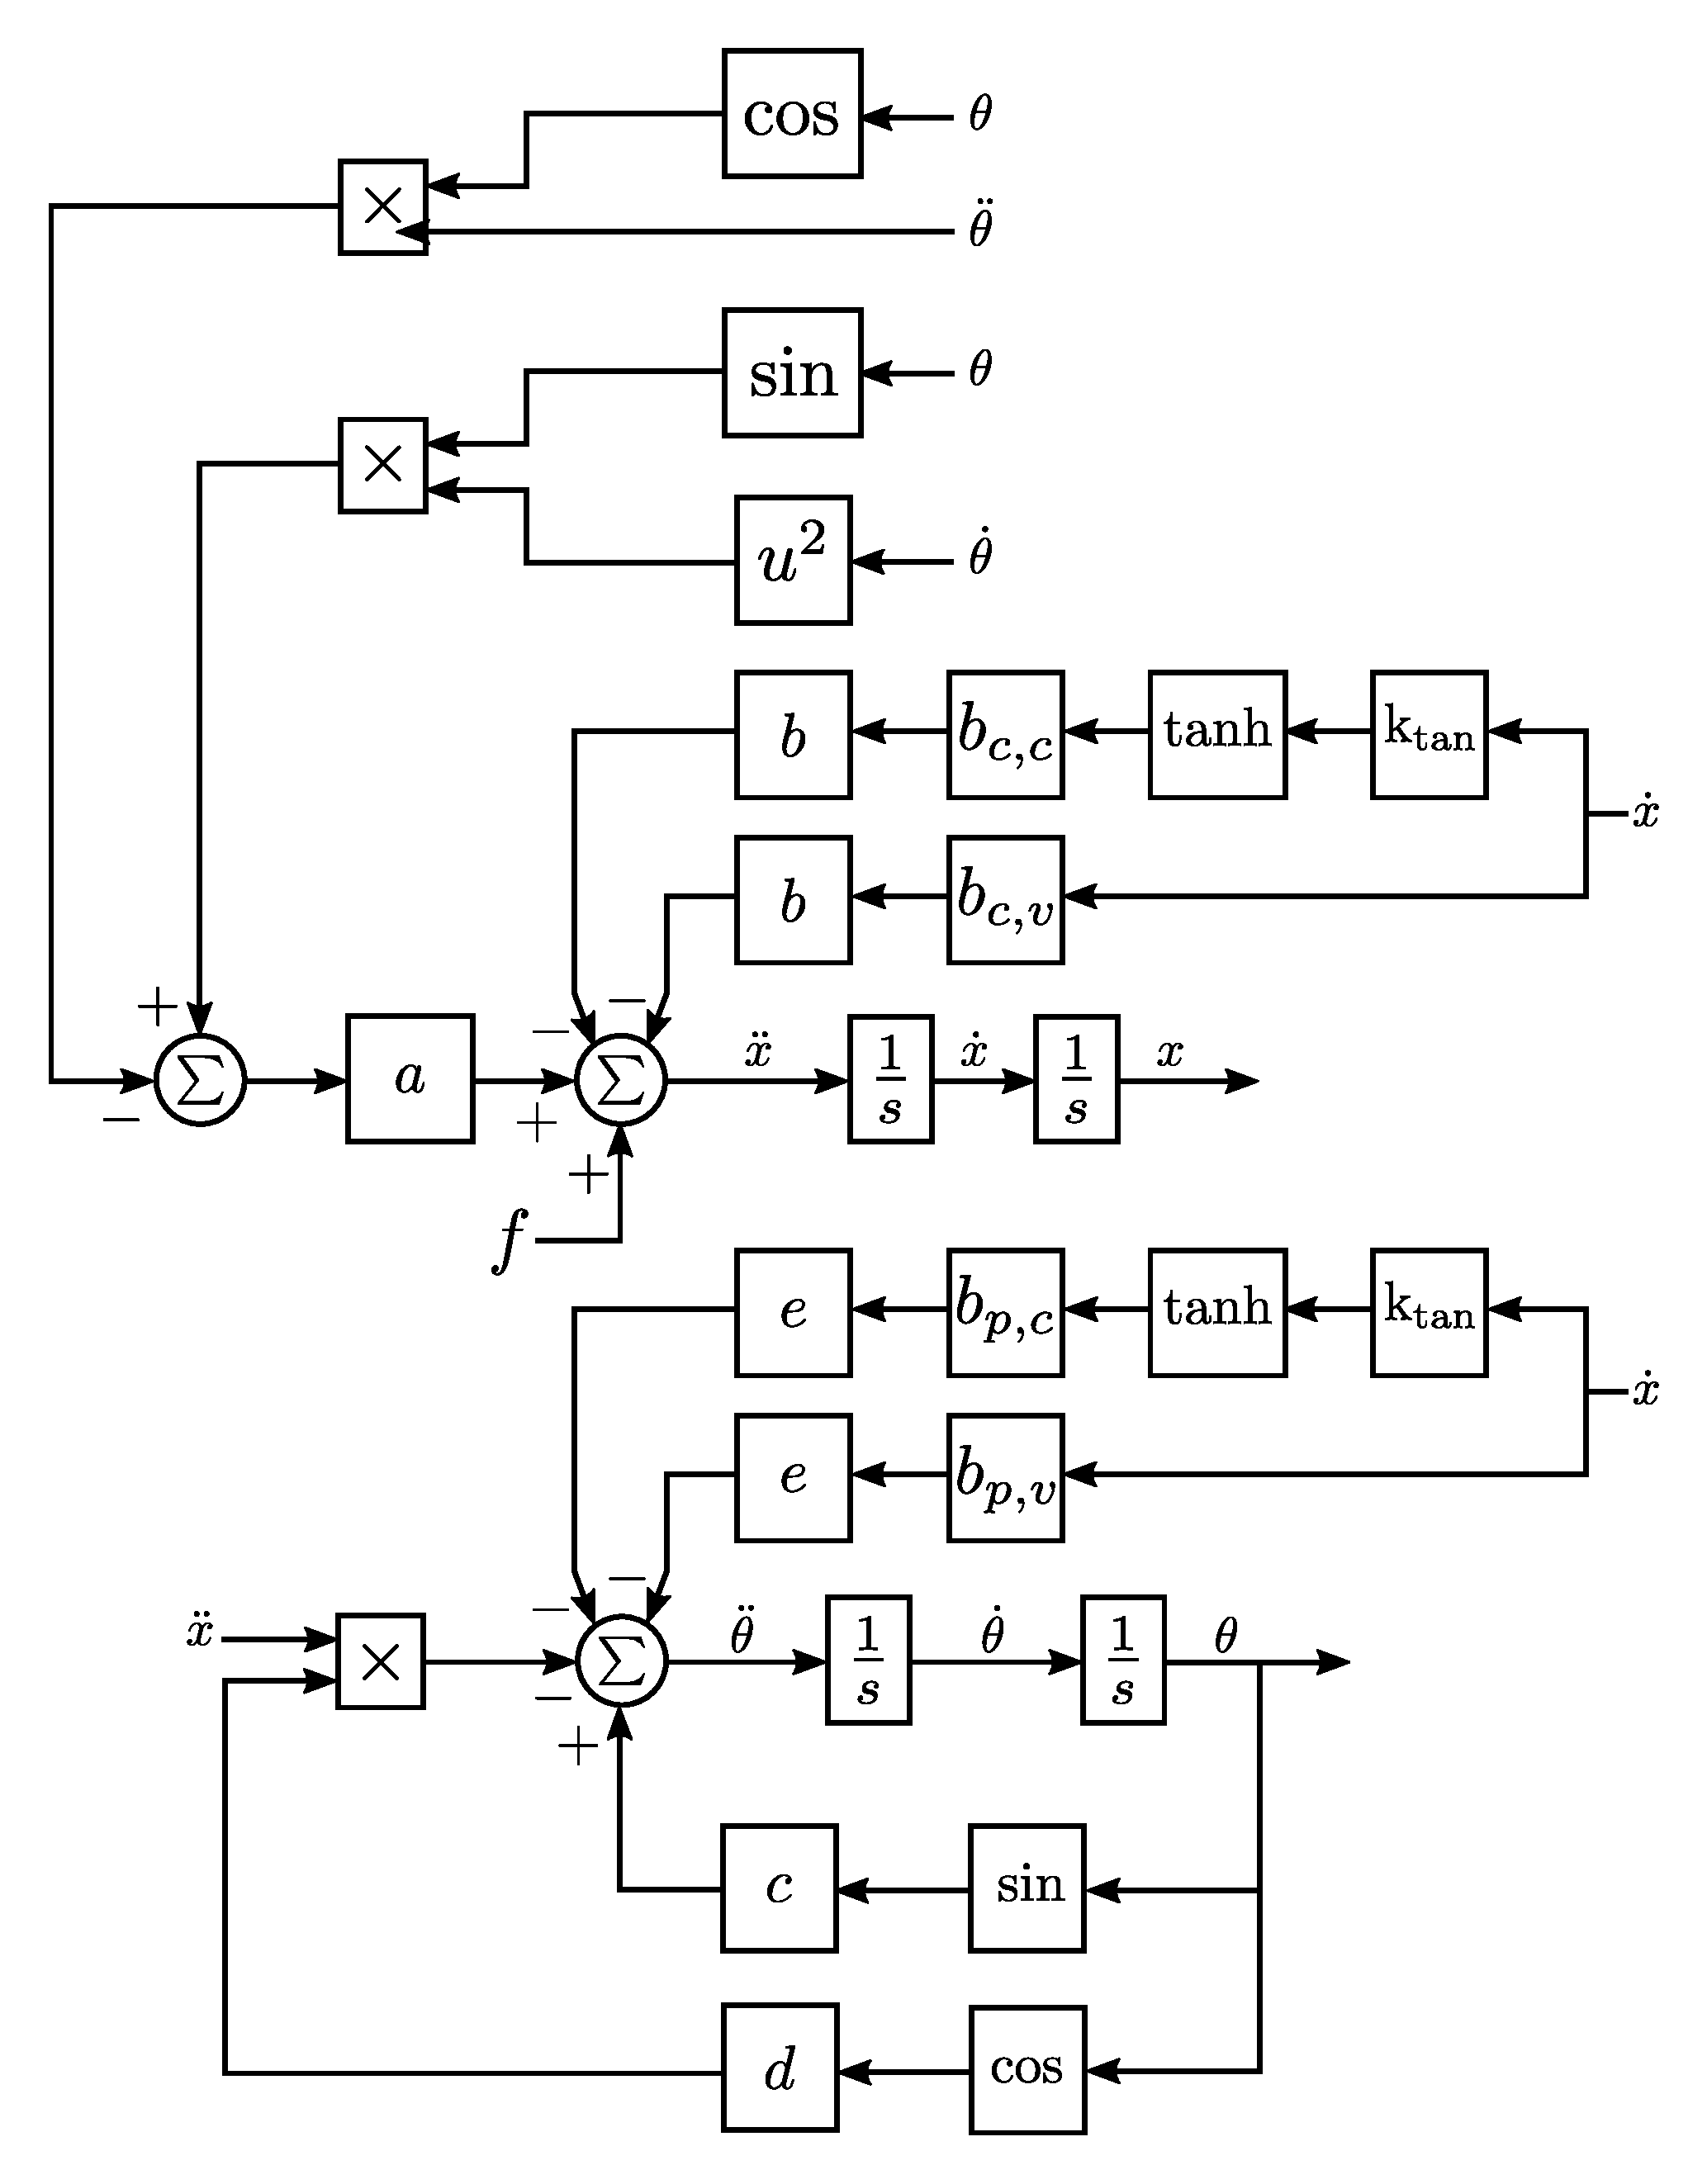
\includegraphics[width=.7\textwidth]{figures/blockDiagramWithFriction}
  \caption{A block diagram derived from the dynamic equations, later used for simulation. Five signal connections, from $\dot{\theta}$, $\ddot{\theta}$, $\ddot{x}$ and two from $\theta$, are drawn without explicit connection to keep the figure clear.}
  \label{fig:blockDiagram}
\end{figure}

This is implemented in Matlab Simulink to simulate the system. A graphical layer, including the obstacles, is added to the simulation to show the system in action.